\documentclass[format=acmlarge]{acmart}

\usepackage{amsmath}
\DeclareMathOperator*{\argmax}{argmax}

\usepackage{hyperref}

\setcopyright{rightsretained}
\copyrightyear{2017}

\begin{document}
\title{Naive Bayesian approach to news headline classification}

\author{Kenneth Allen}
\affiliation{%
  \institution{Armstrong State University}
  \department{Department of Computer Science \& Information Technology}
  \city{Savannah}
  \state{GA}
  \postcode{31419}
  \country{United States of America}}
\email{ka3878@stu.armstrong.edu}

\author{Jeffrey Young}
\affiliation{%
  \institution{Armstrong State University}
  \department{Department of Computer Science \& Information Technology}
  \city{Savannah}
  \state{GA}
  \postcode{31419}
  \country{United States of America}}
\email{jy8672@stu.armstrong.edu}

\begin{abstract}
News article headlines have traditionally been a source of attraction without providing much content.  Traditionally, the information value of headlines has been considered miniscule at best. This research effort tests these preconceived notions of headline information quality as well as the usability of minable headline data.  The efforts of this study began with attaining a set of approximately one million headlines taken from the Australian Broadcasting Corporation.  The data set was processed using a naive Bayes approach to produce both test and training sets.  The training set was used to make predictions of weekend, month, season, year, election time, first chronological half of the data set, prime minister's affiliation, and originating publication.  The study has concluded that quality information can be extracted and features can be predicted with an accuracy well above that of chance.
\end{abstract}

\keywords{Text classification, Naive Bayesian, Headlines, Machine learning}

\maketitle

\section{Background}
\subsection{Bayes' Theorem}
Bayes' Theorem is a simple mathematical formula used for calculating conditional probabilities. It figures prominently in subjectivist or Bayesian approaches to epistemology, statistics, and inductive logic. Subjectivists maintain that rational belief is governed by the laws of probability and lean heavily on conditional probabilities in their theories of evidence and their models of empirical learning. Bayes' Theorem is central to these initiatives both because it simplifies the calculation of conditional probabilities and because it clarifies significant features of subjectivist position. Indeed, the Theorem's central insight that a hypothesis is confirmed by any body of data that its truth renders probable is the cornerstone of all subjectivist methodology.

$$P(A|B) = \frac{P(A) P(B|A)}{P(B)}$$

\subsection{Naive Bayes Classification}
Naive Bayes is a family of algorithms that take advantage of probability theory and Bayes' Theorem to predict the category of a sample (like a piece of news or a customer review). They are probabilistic, which means that they calculate the probability of membership in each category for a given sample, and then output the category with the highest one. The way they get these probabilities is by using Bayes' Theorem, which describes the probability of a feature, based on prior knowledge of conditions that might be related to that feature.

Take a set of classes $C$, a domain $S$, an element $s \in S$, and a set of $s$'s features $a_1, ..., a_n$.  We use simple Laplace smoothing to compensate for some low-probability features occuring zero times in a limited training set.  The classifier is a function $f: S \mapsto C$ defined as such:

$$f(s) = \argmax_{c \in C} P(c|s)$$

$$P(c|s) = \frac{P(c)}{P(s)} P(s|c)$$

$$P(s|c) = \prod_{i = 1}^n P(a_i|c)$$

$$P(a_i|c) = \frac{\textrm{training samples in class with feature} + 1}{\textrm{total training samples in class} + n}$$

\section{Data Processing}
\begin{figure}
  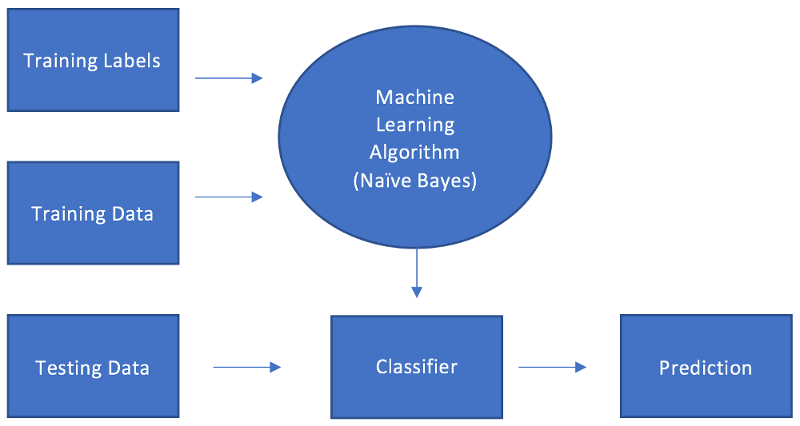
\includegraphics{block-diagram}
  \caption{Block diagram of classifier system.}
  \label{fig:one}
\end{figure}

\subsection{Training Labels}
Labeled corpora may be used to train and evaluate a wide range of learning algorithms. Assigning a label is considered a judgment task performed by a human (worker, judge, expert, annotator, etc.).  Labels for this undertaking were determined exclusively by date and originating publication.

\subsection{Data}
Data used in test and training sets was sourced from two sources.  The first dataset was sourced from the Australian Broadcasting Corporation (\url{http://www.abc.net.au/news/}) and consisted of approximately one million news headlines with corresponding dates.  The second dataset was sourced from Examiner.com (previously at \url{http://www.examiner.com/}) and consisted of approximately three million headlines with corresponding dates.

The first dataset was trained and used to extrapolate weekend, month, season, year, election time, first chronological half of the data set, and current prime minister's party affiliation.  The second dataset was used to train the classifier to distinguish between headlines from two different publications:  a longstanding, public, professional broadcaster and a crowdsourced publishing platform with loose standards.  Essentially, it was being challenged to distingish between news for a regional or global audience, as well as recognizing so-called 'clickbait' designed exclusively to be psychologically enticing.

For each test, 10\% of the data was randomly removed and used as a test set while the remaining 90\% was used as a training set.

\subsection{Naive Bayes Classifier}
The formulas described in the Background section were implemented in Java.  Since the product of so many miniscule fractions can easily underflow an IEEE 64-bit double-precision floating-point number's exponent, the calculations are done using Java's built-in \texttt{BigDecimal} data type, with a precision setting of 32 bits for each of the exponent and significand.

\subsection{Prediction}
Prediction quality was measured with a bevy of statistics.  Accuracy is simple to calculate ($\frac{\textrm{correct classifications}}{\textrm{tested elements}}$), and can be easily compared to the accuracy of a feature-ignorant guess.

For binary criteria, more informative values can be generated.  Use $\mathit{TP}$, $\mathit{FP}$, $\mathit{FN}$, and $\mathit{TN}$, to represent true positives, false positives, false negatives, and true negatives, respectively.  Especially important are true positive rate ($\mathit{TPR} = \frac{\mathit{TP}}{\mathit{TP} + \mathit{FN}}$), true negative rate ($\mathit{TNR} = \frac{\mathit{TN}}{\mathit{FP} + \mathit{TN}}$), positive predictive value ($\mathit{PPV} = \frac{\mathit{TP}}{\mathit{TP} + \mathit{FP}}$), and negative predictive value ($\mathit{NPV} = \frac{\mathit{TN}}{\mathit{FN} + \mathit{TN}}$).

\begin{figure}
  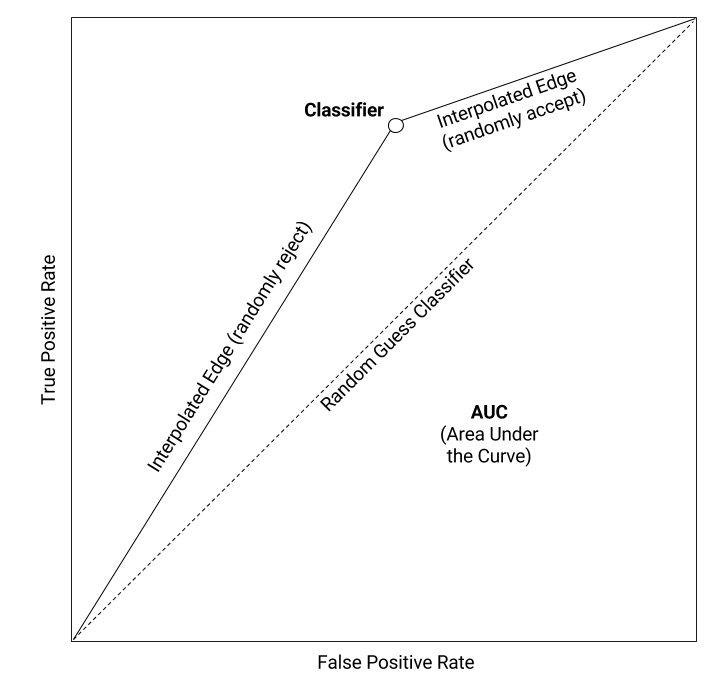
\includegraphics{interpolated-roc}
  \caption{Interpolated Receiver Operating Characteristic.}
  \label{fig:two}
\end{figure}

The Naive Bayesian Classifier does not have a sensitivity parameter, so it only creates one point on a Receiver Operating Characteristic (ROC) graph.  We can trivially interpolate between that point and the points $(0, 0)$ and $(1, 1)$ by imagining a series of classifiers that randomly choose with a certain probability whether to refer to our classifier or to automatically reject or accept, respectively (as in Fig. 2).  (This is equivalent to 'convex hull' techniques, but for a single data point.)  In this way, we get a curve and can calculate the area under it simply as $\mathit{AUC} = \frac{\mathit{TPR} + \mathit{TNR}}{2}$.  The $F_1$ score is calculated as the harmonic mean of $\mathit{TPR}$ and $\mathit{PPV}$:

$$F_1 = \frac{2}{\frac{1}{\mathit{TPR}} + \frac{1}{\mathit{PPV}}}$$

\section{Results and Performance}

\begin{table}
  \caption{Classifier Results}
  \label{tab:one}
  \begin{tabular}{|p{10em}|l|l|l|l|l|}
    \hline
    Criterion & Dataset & Accuracy & Blind Guess & ROC-AUC & $F_1$ score\\
    \hline
    publication month & ABC & 0.169 & 0.083 & - & -\\
    \hline
    publication season & ABC & 0.346 & 0.250 & - & -\\
    \hline
    publication year & ABC & 0.225 & 0.067 & - & -\\
    \hline
    first chronological half & ABC & 0.710 & 0.500 & 0.710 & 0.717\\
    \hline
    published on weekend & ABC & 0.816 & 0.592 & 0.619 & 0.356\\
    \hline
    published in 90 days \newline before natl. election & ABC  & 0.916 & 0.861 & 0.508 & 0.047\\
    \hline
    published under Labor \newline Party Prime Minister & ABC  & 0.648 & 0.508 & 0.634 & 0.563\\
    \hline
    original publication & ABC \& Examiner.com & 0.931 & 0.617 & 0.912 & 0.953\\
    \hline
  \end{tabular}
\end{table}

Table 1 gives a summary of the performance of the classifier given different labeling criteria, on a partial and full headline dataset.  The actual Accuracy can be compared favorably to a Random Guess, which is made only with the knowledge of the relative class frequencies (for instance, guessing an article was published on a weekend with a probability of $\frac{2}{7}$ or on a weekday with a probability of $\frac{5}{7}$).  The ROC-AUC (Area Under the Curve of the Interpolated Receiver Operating Characteristic) and $F_1$ score, as described above, also give meaningful insight.  (The $F_1$ scores presented are for the 'positive' conditions; the value for the 'negative' condition would be different.)

\begin{table}
  \caption{Most Indicative Words}
  \label{tab:two}
  \begin{tabular}{r|ll|ll}
    Rank & 'ABC' Word & Explanation & 'Examiner.com' Word & Explanation\\
    \hline
    1 & qld & Abbreviation for Queensland & year-old & Human-interest stories\\
    2 & nsw & Abbreviation for New South Wales & ncaa & College basketball\\
    3 & nrn & Rural Australia news section & mom & Stories for \& about mothers\\
    4 & australias & Originating country & spoilers & Story details of movies/TV\\
    5 & bendigo & Australian city and bank & rumors & Gossip stories\\
    6 & townsville & Australian city & dwts & 'Dancing with the Stars', a TV show\\
    7 & gippsland & Australian region & honors & Headlines about awards\\
    8 & bikie & Australian slang for "biker" & dlc & 'Downloadable content', a videogame term\\
    9 & aust & Abbreviation for Australia & gluten-free & Health/diet craze\\
    10 & bushfire & Australian term for "wildfire" & moms & Stories for \& about mothers\\
  \end{tabular}
\end{table}

All of our classifier configurations outperformed random guessing by a significant margin.  Perhaps our most significant result comes when we try to use machine learning to sort the full set of four million headlines between their originating publications.  We can delve into the internals of the collated data for more insight:  Table 2 presents the words most strongly identified with each of the ABC and Examiner.com.  They scored highest in a formula that compares the effect in our Laplace-smoothed Bayesian equations:

$$\textrm{score}(\textrm{word}, \textrm{class}) = \frac{1 + \textrm{instances of word in class}}{(\textrm{number of classes} - 1) + \textrm{instances of words in all other classes}}$$

\section{Discussion}
From the test results, it can be concluded that news headline data has a greater amount of informational value than previously assumed.  This study has concluded that it is possible to extrapolate usable information in regard to a multitude of inquiries.  Also, the approach outlined in this report can be used to predict the informational quality of the underlying article of which the headline represents.

\section{Works Cited}
\begin{itemize}
\item A practical explanation of a Naive Bayes classifier. (2017, October 03). Retrieved October 09, 2017, from https://monkeylearn.com/blog/practical-explanation-naive-bayes-classifier/
\item Joyce, J. (2003, June 28). Bayes' Theorem. Retrieved October 09, 2017, from https://plato.stanford.edu/entries/bayes-theorem/
\item A simple explanation of Naive Bayes Classification. (n.d.). Retrieved October 10, 2017, from https://stackoverflow.com/questions/10059594/a-simple-explanation-of-naive-bayes-classification\#20556654
\item Mitchell, T. M. (2015). Machine learning. Johanneshov: MTM.
\end{itemize}

\end{document}